\documentclass{article}
\author{Magnus Bergkvam}
\title{Project 1 \\ FYS-STK3155}
\usepackage{url}
\usepackage{amsmath}
\usepackage{graphicx}
\usepackage{subfig}
\usepackage{bm}
\graphicspath{{../figures/}}

% Julia code configuration
\usepackage[usenames,dvipsnames]{color} % more flexible names for syntax highlighting colors
\usepackage{listings}
\lstdefinelanguage{julia}
{
  keywordsprefix=\@,
  morekeywords={
    exit,whos,edit,load,is,isa,isequal,typeof,tuple,ntuple,uid,hash,finalizer,convert,promote,
    subtype,typemin,typemax,realmin,realmax,sizeof,eps,promote_type,method_exists,applicable,
    invoke,dlopen,dlsym,system,error,throw,assert,new,Inf,Nan,pi,im,begin,while,for,in,return,
    break,continue,macro,quote,let,if,elseif,else,try,catch,end,bitstype,ccall,do,using,module,
    import,export,importall,baremodule,immutable,local,global,const,Bool,Int,Int8,Int16,Int32,
    Int64,Uint,Uint8,Uint16,Uint32,Uint64,Float32,Float64,Complex64,Complex128,Any,Nothing,None,
    function,type,typealias,abstract
  },
  sensitive=true,
  morecomment=[l]{\#},
  morestring=[b]',
  morestring=[b]" 
}
\lstset{
basicstyle=\ttfamily, 
columns=fullflexible, % make sure to use fixed-width font, CM typewriter is NOT fixed width
numbers=left, 
numberstyle=\small\ttfamily\color{Gray},
stepnumber=1,              
numbersep=10pt, 
numberfirstline=true, 
numberblanklines=true, 
tabsize=4,
lineskip=-1.5pt,
extendedchars=true,
breaklines=true,        
keywordstyle=\color{Blue}\bfseries,
identifierstyle=, % using emph or index keywords
commentstyle=\sffamily\color{OliveGreen},
stringstyle=\color{Maroon},
showstringspaces=false,
showtabs=false,
upquote=false,
texcl=true % interpet comments as LaTeX
}
\lstset{
literate={σ}{{$\sigma$}}1
{λ}{{$\lambda$}}1
}
% End julia code

\begin{document}
\maketitle
\bibliographystyle{unsrt}

\section{Abstract}
We have in this project fitted various models on data generated from the
franke-function, a function which somewhat resembles a landscape, as well as real-world
geographical data. In both cases we have used polynomial features up to order
$5$ related to a position in the "landscape" in some way. For the
franke-function we have used both response with and without added noise, and for
the landscape data we naturally have some stochastic noise built in. The models
we looked at was ridge, lasso and ordinary least squares.  For both the
mean-squared-error and the $R^2$ score we saw that for the franke-function
without noise the models performed rather similarly, but when we added noise
simpler versions of ols and quite heavily penalized ridge/lasso models performed
much better than the more complex models, while the same couldn't be said for
the data-rich landscape data.  Throughout the project we have clearly seen that
less complex models often perform better when we have some added noise (at least
in the case when we have somewhat limited data), but that this is not the case
when there is no noise (or a very high signal to noise-ratio). We have also
explored how this result is tied to the bias-variance tradeoff, and manifested
the importance this has for choosing a correct model complexity for our given
data.

\section{Introduction}
Linear regression often is seen as a rather simple machine-learning method in
itself, but we do have less complex models than this again. Choosing the right
model complexity is well known as being an important part in getting the best
possible models for prediction, and in a lot of applications linear regression
offers just the right amount of complexity needed. Especially with cases where
our data is limited, or we have a low signal-to-noise ratio, linear regression
often performs very well \cite[p.~43]{hastie2009elements}. \\

However, when can it become beneficial to choose even less complex models than
this again? This is mainly what this project is about. We will mainly base this
project around the franke-function, which is a 2-dimensional function which
somewhat resembles a landscape \cite{franke2ddesc}. On the franke-function we
will fit ordinary least squares linear regression with polynomial features up to
order $5$ (with interactions), and then compare these results (using mainly the
mean squared error and $R^2$ metrics) to ridge and lasso regression on the
same data. We will also explore the performances of these models on some
real-world geographical data as well. For the franke-function we will be
generating two vectors of random points in $\left[ 0, 1 \right]$, and use
polynomial features with interactions of order $5$ for our data, for all our
models. We will also try to tie the results we get to the well-known
bias-variance tradeoff in machine learning, and on our way there explore various
resampling techniques for getting better estimates for model performances.
\\

We now get into a description of the models/methods we have used, before we present the
results and finally conclude what we have found out.

\section{Methods}
\subsection{The franke function}
The franke-function is a function of two variables with the following definition:
\begin{align*}
    f(x,y) & = \frac{3}{4}\exp{\left(-\frac{(9x-2)^2}{4} - \frac{(9y-2)^2}{4}\right)}+\frac{3}{4}\exp{\left(-\frac{(9x+1)^2}{49}- \frac{(9y+1)}{10}\right)} \\
           & +\frac{1}{2}\exp{\left(-\frac{(9x-7)^2}{4} - \frac{(9y-3)^2}{4}\right)} -\frac{1}{5}\exp{\left(-(9x-4)^2 - (9y-7)^2\right) }
\end{align*}
We will use this function to generate a response from two explanatory variables
$x_1$ and $x_2$ both of which will be drawn randomly from $\left[ 0, 1 \right]$.
To get a visual picture of what the franke-function looks like on $\left[ 0, 1
        \right] \times \left[ 0, 1 \right]$ see figure \ref{franke-function-plot}.

\begin{figure}
    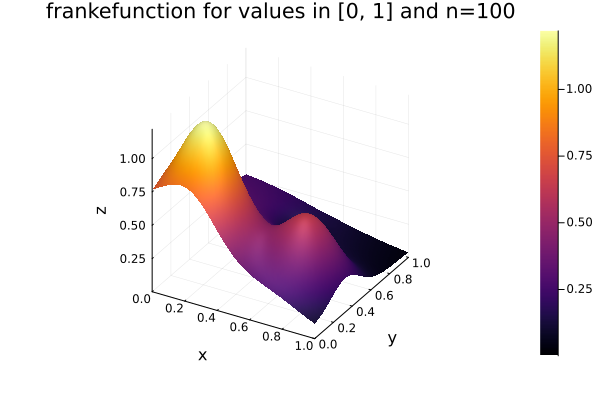
\includegraphics[scale=0.5]{frankefunction}
    \caption{A surface plot of the franke-function on $\left[ 0, 1 \right] \times \left[ 0, 1 \right]$}
    \label{franke-function-plot}
\end{figure}

Looking at such a plot we can see that the franke-function does somewhat
resemble a terrain. We will use the franke-function to generate data, both with
and without noise.  In the case without noise we will simply get the
following response:
$$\mathbf{y} = f(\mathbf{x_1}, \mathbf{x_2})$$
(Here where $f$ is applied element-wise to $\mathbf{x1}$ and $\mathbf{x2}$).
With noise we simply get:
$$\mathbf{y} = f(\mathbf{x_1}, \mathbf{x_2}) + \mathbf{\epsilon}$$
Where in this case $\epsilon_i \sim N(0, \sigma^2)$. We will use $\sigma = 0.1$
throughout all of our calculations (but this is easily adjustable in the code).

\subsection{Geographical data}
As mentioned, another source for data which was used for analysis of the
different models is some real-world geographical data. The data is stored as a
tiff image file and consists simply of a set of numerical values in a square
grid, where the numerical value indicates the height of the terrain in some way.
Figure \ref{landscape-plot} contains a plot of the data which we have used for
our analysis here.  The data is gathered from
\url{https://earthexplorer.usgs.gov/}, and we have here downloaded a region
around \textit{Møsvatn Austfjell} in Norway. This data includes a lot of
datapoints ($3601\times 1801 = 6485401$ to be exact), which is quite a lot more
than we need to fit a good model. Trying to fit a lot of different models to
such a big amount of data will often take a lot of memory and processing power,
so for this sake I have throughout our calculations limited the data to look at
only the first $400\times 500 = 20000$ observations, which should be more than
enough for our case. When reading the tiff-file we only get a matrix of values
out, but we will look at this as an image, and then use the position of the
response in the matrix as explanatory variables for our model. In other words,
if say the fifth pixel in the fourth row has the value $10^{-5}$, the response
will obviously be $10^{-5}$, while the two explanatory variables will have
values $5$ and $4$ (originally that is, but we will scale these and add
interactions and so on).  This way we will be able to gather data whose
structure closely resembles that of the franke-function. We can then use the
same techniques to set up a design-matrix and a response, as we do with the
franke-function.

\begin{figure}
    \centerline{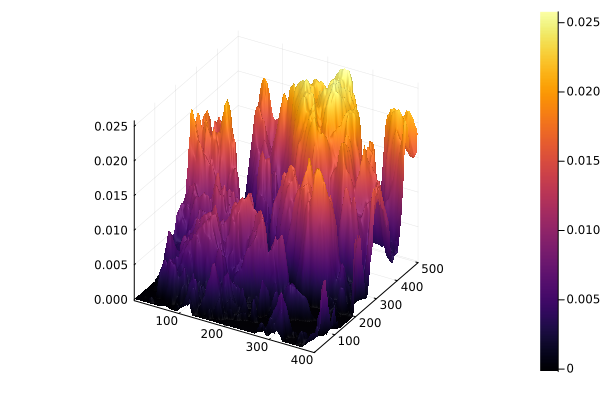
\includegraphics[scale=0.5]{landscapesurface}}
    \caption{A surface plot of the landscape data we have used. Keep in mind
        here that the axis here is simply the index of each datapoint in the
        tiff-file. This means that the axis here doesn't really tell us much, but
        shows the overall structure of the terrain nonetheless.}
    \label{landscape-plot}
\end{figure}

\subsection{Data/Data scaling}
The data and design matrix used throughout the project is mostly the same for
the different models we fit the data to. As previously mentioned, for the
franke-function the data we have used is simply a collection of two randomly
generated datapoint-vectors $\mathbf{x}_1$ and $\mathbf{x}_2$, each of size
$200$ (for the most part), and the response is simply the value of the
franke-function evaluated at some point (plus some added noise in some cases).
When we added noise we have drawn this from the normal distribution with mean
$0$ and standard-deviance $0.1$, which satisfies a common assumption for linear
regression models \cite[s.~1.4.5]{murphy2012machine}. We have chosen to use a
standard-deviance of $0.1$ in order to not have too low of a
signal-to-noise-ratio (the franke-function usually returns quite low values as
one can can see from figure \ref{franke-function-plot}). For the geographical
data we load the data in from a tiff file of geographical data, but the setup of
the design matrix is exactly the same, with the difference being that the
$x_1$s, $x_2$s and the response have been drawn directly from the tiff-file.
For the setup of the design-matrix of for example fifth order polynomial features we have
included in the first column the first-order values of the $x_1$s, the second
column the second-order values of $x_1$s, and so on up to the fifth order.  The
sixth to tenth column then is the first to fifth order terms of $x_2$s and then
the rest of the $4 \cdot 4 = 16$ columns is for interaction terms between the
two variables. The same structure applies of course to other orders as well. One
exception to this exact setup of design-matrix is for ordinary least squares
where we have added an intercept by setting the first column to consist of only
$1$s.
\\
Throughout the whole of this project we have scaled the features of the matrix,
simply by centering the mean around $0$ and scaling by the standard deviance.
This way we have that each feature is $1$ away from $0$ on average. In the case
of ordinary least squares regression this scaling is not important for model
performance, as the model will be able to scale the $\beta$s depending on the
scaling of the features and give the same minimization of the loss-function
(just with different parameters $\beta$).  However, in the case of ridge/lasso
regression which both include a penalty term, it becomes important to scale the
data so that the scale of the data doesn't affect how much we penalize the
parameters (more about this in the ridge/lasso section at
\ref{ridge-lasso-model-sec}).
\\
A last thing of note we have used throughout the project is train-test-splitting
(except when doing cross-validation). We then split our data into a train set
consisting of $80\%$ of the datapoints, and $20\%$ of the data for testing.
This lets us evaluate how well our model performs on "new" data, i.e. data the
model has not been trained on. The reason this is important is in order for us
to recognize overfitted models, which often become the case when we have a
higher model complexity \cite[s.~7.2]{hastie2009elements}. In such cases we
could have a model that predicts the training data very well, but generalizes
very poorly to new data.  For the franke-function I have written a function
\textbf{generatedata} which takes hand of all of the mentioned above (I am using
Julia for all the code in this project). It is a bit long, but well worth
inclusion here as it is central to all of the programs that use the
franke-function:
\begin{lstlisting}[language=julia]
# Generate a design matrix consisting of random x-s (two explanatory variables)
# with a polynomial of a given order (we will use order 5 for our analysis
# mainly). Additionally includes options for adding intercept column, noise,
# number of observations and random seed.
function generatedata(order::Int64; split=true, include_intercept=false, add_noise=false, noise_σ=0.1, n=200, custom_seed=1000)
    # Setting the seed for train test splitting and random x1/x2
    seed!(custom_seed)

    # Generating x-s
    x1 = rand(n)
    x2 = rand(n)

    # Creating the design matrix
    X = generatedesignmatrix(x1, x2, order)

    # Creating the response
    y = Functions.frankefunction(x1, x2)


    # Shuffle before train-test splitting
    Xs, ys = shufflematrices(X, y)

    # Train-test splitting
    if !split
        return standardscale(Xs, Xs), ys
    end
    indextosplitat = Int(floor(size(Xs, 1) * 0.8))
    X_train, X_test = Xs[1:indextosplitat, :], Xs[(indextosplitat+1):size(Xs, 1), :]
    y_train, y_test = ys[1:indextosplitat, :], ys[(indextosplitat+1):size(ys, 1), :]

    # Scaling X\_train/X\_test
    # We use the column means from the original X\_train to subtract from the
    # columns in X\_test. We must do this before we scale the X\_train
    X_test = standardscale(X_test, X_train)
    # We then can scale the X\_train
    X_train = standardscale(X_train, X_train)

    if add_noise
        # Add response with noise
        y_train += rand(Normal(0, noise_σ), length(y_train))
        y_test += rand(Normal(0, noise_σ), length(y_test))
    end

    if include_intercept
        X_train = [ones(size(X_train, 1)) X_train]
        X_test = [ones(size(X_test, 1)) X_test]
    end

    return X_train, X_test, y_train, y_test
end
\end{lstlisting}

Keep in mind here that we are using the features of the training-set to scale
the features of the test-set. We have also used some other local functions like
\textbf{standardscale} (scaling as described before) and
\textbf{shufflematrices} (randomly shuffles rows in a matrix), which their
implementation is rather trivial (but of course feel free to see exactly how
they are implemented by looking at the full source-code at:
\url{https://github.com/magnouvean/ml-physics-projects/tree/main/project1/julia}).
We also here use \textbf{generatedesignmatrix}, which I'll include the
implementation of the here, as it is a little more complicated, and very central
for all the calculations we have done (including setting up the landscape data):
\begin{lstlisting}[language=julia]
# Generate a matrix with features as polynomial terms with interactions
function generatedesignmatrix(x1, x2, order)
    X = zeros((length(x1), 2 * order + (order - 1)^2))
    for i in 1:order
        X[:, i] = x1 .^ i
        X[:, order+i] = x2 .^ i
    end
    for i in 1:(order-1)
        for j in 1:(order-1)
            X[:, 1+order+i*(order-1)+j] = (x1 .^ i) .* (x2 .^ j)
        end
    end

    return X
end
\end{lstlisting}

Shuffling the data is perhaps not nessecary here in the case of the
franke-function seeing as the explanatory variables are randomly drawn (but I
have done so anyway just out of good practice), however in the case of the
landscape data this is very important, as here the data is sorted when reading
the data in, and if we then do not shuffle the data before, and we apply
train-test-splitting, we will get different regions of our response for the
training and testing data, in other words, the model will be trained on data
from some area and tested on data from another area, which will then probably
give quite poor performance (unless the two regions the train-data and test-data
are gathered from are very similar).

\subsection{Metrics}
We will mainly use two different metrics in our analysis. The perhaps most
central one is the mean squared error, and the other one is the $R^2$ score.
Given some response $\mathbf{y}$ with $n$ values and some predictions for
$\mathbf{y}$, $\hat{\mathbf{y}}$ the mse is given as: \cite{week34notes}
$$MSE(\mathbf{y}, \hat{\mathbf{y}}) = \frac{1}{n} \sum_{i=1}^n (y_i - \hat{y}_i)^2$$
while the $R^2$ score is given by: \cite{week34notes}
$$R^2(\mathbf{y}, \hat{\mathbf{y}}) = 1 - \frac{\sum_{i=0}^{n-1} (y_i - \hat{y}_i)^2}{\sum_{i=0}^{n-1}(y_i - \overline{y})^2}$$

\subsection{Ordinary least squares}
The first, and conceptually simplest, model we looked at in this project was the
ordinary least squares linear regression. Before we go deeper into this
method, denote $\mathbf{X}$ as our design-matrix and $\mathbf{y}$ as our
response. We assume the following relationship:
$$\mathbf{y} = \mathbf{X} \bm{\beta} + \bm{\epsilon}$$
Where $\bm{\epsilon}$ is some stochastic noise.
We want to include a intercept for our model, and thus we let the first column
in the design matrix $\mathbf{X}$ consist of only $1$s. Ordinary least squares
regression finds the $\bm{\beta}$ which minimizes the loss-function over the
training-data (this optimal value we call $\hat{\bm{\beta}}$) given like:
$$C(\bm{\beta}) = (\mathbf{y} - \mathbf{X}_{train} \bm{\beta})^T (\mathbf{y} - \mathbf{X}_{train} \bm{\beta})$$
Then we get the least squares estimate for $\hat{\bm{\beta}}_{ols}$ given by \cite[s.~3.2]{hastie2009elements}:
$$\hat{\bm{\beta}}_{ols} = (\mathbf{X}^T_{train} \mathbf{X}_{train})^{-1} \mathbf{X}^T_{train} \mathbf{y}_{train}$$
We then can make predictions for the training-set by:
$$\hat{\mathbf{y}}_{train} = \mathbf{X}_{train} \hat{\bm{\beta}}_{ols}$$
and for the test set:
$$\hat{\mathbf{y}}_{test} = \mathbf{X}_{test} \hat{\bm{\beta}}_{ols}$$

\subsection{Ridge and lasso}
\label{ridge-lasso-model-sec}
Ridge and lasso is in lots of ways very similar to ordinary least squares
regression. The setup of the model is exactly the same, i.e. we again have:
$$\mathbf{y} = \mathbf{X} \bm{\beta} + \bm{\epsilon}$$
The difference arises with the cost function we minimize to estimate the parameters. For ridge we use:
$$C(\bm{\beta}) = \left(\sum_{i=1}^{n} (y_i - \beta_0 - \beta_1 x_{i 1} - \dots - \beta_{p} x_{i p})\right) + \lambda \sum_{i=1}^p \beta_i^2$$
and for lasso:
$$C(\bm{\beta}) = \left(\sum_{i=1}^{n} (y_i - \beta_0 - \beta_1 x_{i 1} - \dots - \beta_{p} x_{i p})\right) + \lambda \sum_{i=1}^p \lvert \beta_i \rvert$$
for some hyperparameter $\lambda$, which determines how much we want to penalize
high parameter values. For ridge we get the following estimator \cite[s.~3.4]{hastie2009elements}:
$$\hat{\bm{\beta}}_{ridge} = (X^T X + \lambda I)^{-1} X^T y$$
Also, keep in mind that we do not here penalize the intercept
in the loss-function. We often do this because we in general are ok with a
somewhat high intercept, because this often lead to better performance. We will
therefore when writing our code, fit ridge regression without a intercept (by
not including a first column of only $1$s), and then based on the other
parameters calculate the intercept $\beta_0$ which leads to the optimal
loss. This we calculate this by the following relationship:
$$\beta_0 = \frac{1}{n} \sum_{i=0}^{n-1} y_i - \frac{1}{n} \sum_{i=0}^{n-1} \sum_{j=1}^{p-1} X_{i j} \beta_j$$
, as proved in \cite[s.~Further manipulations]{week35notes}. To get our
estimate we simply replace our $\beta_i$s with their estimates. For
lasso-regression we will use scikit-learns implementation, which takes care of
this for us. Furthermore, from the loss-function expressions we see why it is
important to scale the data beforehand. If we for example have a feature that is
not scaled and takes very low values, the corresponding $\beta$ which
minimizes the first sum (the ols loss) will typically be quite high. This would
then result in this $\beta$ to be penalized quite a lot. If we then scale the
feature to another unit (by for example multiplying with some big number), so
that the feature takes much higher values the corresponding $\beta$ which
minimizes the first sum would then become a lot smaller. This would mean that
this parameter would be much less penalized. In other words we see that the
scaling of the different features will decide how much its corresponding
parameter will be penalized, and this is not something we want. In order to
hinder this happening it is important to scale the features somewhat alike, so
that the scale the features does not determine which parameters will be shrunk
a lot, and which will be shrunk less.

\subsection{The bias variance tradeoff}
Central in this project will be the bias variance tradeoff, as this is the reason
why ridge and lasso often can give better predictions than ordinary least
squares. We will here derive the bias-variance equation. Consider the model
$\mathbf{y} = f(\mathbf{x}) + \bm{\epsilon}$ where $E(\bm{\epsilon}) = 0$ and
$Var(\bm{\epsilon}) = \sigma^2 \mathbf{I}$, for some function $f$. The job in machine-learning
is to estimate this $f$. We call $\hat{f}$ some estimate of this function $f$.
We then get $\hat{\mathbf{y}} = \hat{f}(\mathbf{x})$, which is some prediction.
We consider the squared error of one such prediction $(y - \hat{y})^2$. We
now want to find an expression for this squared error as this is what the
MSE statistic approximates. However this is a little difficult to calculate as
both terms here are stochastic. We therefore calculate the expectance of this
expression, in which we get:
\begin{align*}
    E((y - \hat{y})^2) & = E((f(x) + \epsilon - \hat{f}(x))^2)                                                      \\
                       & = E((\epsilon + (f(x) - \hat{f}(x)))^2)                                                    \\
                       & = E(\epsilon^2 + 2\cdot \epsilon \cdot (f(x) - \hat{f}(x)) + (f(x) - \hat{f}(x))^2)        \\
                       & = E(\epsilon^2) + 2\cdot E(\epsilon) \cdot E(f(x) - \hat{f}(x)) + E((f(x) - \hat{f}(x))^2) \\
                       & = E((\epsilon - E(\epsilon))^2) + E((f(x) - \hat{f}(x))^2)                                 \\
                       & = \sigma^2 + E((f(x) - \hat{f}(x))^2)                                                      \\
\end{align*}
Here we have used independence of $\epsilon$ from $f(x) - \hat{f}(x)$ which
stems from the fact that we may assume that $\hat{f}(x)$ and $\epsilon$ are
independent. We now focus on calculating the second part of this, i.e. $E((f(x)
    - \hat{f}(x))^2)$. We have:
\begin{align*}
     & E\left[(f(x) - \hat{f}(x))^2\right]                                                                                                                                                \\
     & = E\left[((f(x) - E(\hat{f}(x))) + (E(\hat{f}(x)) - \hat{f}(x)))^2\right]                                                                                                          \\
     & = E\left[(f(x) - E(\hat{f}(x)))^2 + 2\cdot (f(x) - E(\hat{f}(x))) \cdot (E(\hat{f}(x)) - \hat{f}(x)) + (E(\hat{f}(x)) - \hat{f}(x))^2\right]                                       \\
     & = E\left[(f(x) - E(\hat{f}(x)))^2\right] + 2\cdot E\left[(f(x) - E(\hat{f}(\mathbf{x}))) \cdot (E(\hat{f}(x)) - \hat{f}(x))\right] + E\left[(E(\hat{f}(x)) - \hat{f}(x))^2 \right] \\
     & = (f(\mathbf{x}) - E(\hat{f}(x)))^2 + 2\cdot \left(f(x) - E(\hat{f}(x))\right) \cdot E\left[(E(\hat{f}(x)) - \hat{f}(x))\right] + E\left[(E(\hat{f}(x)) - \hat{f}(x))^2 \right]    \\
     & = (f(\mathbf{x}) - E(\hat{f}(x)))^2 + 2\cdot \left((f(x) - E(\hat{f}(x)))\right) \cdot (E(\hat{f}(x)) - E(\hat{f}(x))) + E\left[(E(\hat{f}(x)) - \hat{f}(x))^2 \right]             \\
     & = (E(\hat{f}(x)) - f(x))^2 + E\left[(\hat{f}(x) - E(\hat{f}(x)))^2 \right]                                                                                                         \\
\end{align*}
Typically in machine learning we call the first term here the squared bias of the
model, and the second term the variance. In total we get:
$$E((y - \hat{y})^2) = \sigma^2 + (E(\hat{f}(x)) - f(x))^2 + E\left[(\hat{f}(x) - E(\hat{f}(x)))^2\right] = \sigma^2 + Bias(\hat{f}(x))^2 + Var(\hat{f}(x))$$
In vector form this becomes:
$$E((\mathbf{y} - \hat{\mathbf{y}})^T (\mathbf{y} - \hat{\mathbf{y}})) = \sigma^2 + Bias(\hat{f}(\mathbf{x}))^2 + Var(\hat{f}(\mathbf{x}))$$
We see that the expected squared prediction error is given as a sum of the
variance of the noise $\sigma^2$, the bias of our model, and the variance of our
model. Here $\sigma^2$ is an irreducible part we cannot control by the choice of
our model, while the bias and variance is dependent on the type of model that we
use \cite[s.~2.9]{hastie2009elements}. We can see here that the bias is the
difference between our models' expectation and the actual expectation $f(\mathbf{x})$.
The variance says how much the model varies in predictions when trained on
different data. Typically we have that the more complex the model we have the
lower the bias will be, but we also typically have a higher variance \cite[fig.~2.11]{hastie2009elements}.
We also have that the more observations we have the lower the variance usually
becomes. Both of these concepts are very central for all our results.  We now go
more into detail of this for the models we use in the project.

\subsection{Bias and variance of ols/ridge/lasso}
To explain the bias and variance of the different models, we will dedicate this
section to calculate bias and variance for the parameters in ols and ridge
regression. Lasso regression is more complicated to do these analysis for as we
do not have an analytical expression for $\hat{\bm{\beta}}$, so we will skip
this here. For all our models we usually assume that:
$$y_i = \mathbf{X}_{i *} \bm{\beta} + \epsilon_i$$
With $\epsilon_i \sim N(0, \sigma^2)$, and $\mathbf{X}_{i *}$ being the $i$-th
row in the design-matrix. We will start by looking at some properties of our
response $\mathbf{y}$. Looking first at the expectance of $y_i$ it is easy then to
see:
\begin{align*}
    E(y_i) & = E\left[ \mathbf{X}_{i *} \bm{\beta} + \epsilon_i \right]                 \\
           & = E\left[ \mathbf{X}_{i *} \bm{\beta} \right] + E\left[ \epsilon_i \right] \\
           & = \mathbf{X}_{i *} \bm{\beta} + 0                                          \\
           & = \mathbf{X}_{i *}\bm{\beta}
\end{align*}
(Here we have used the fact that $\mathbf{X}_{i *} \bm{\beta}$ is
non-stochastic and $E(\epsilon_i) = 0$). Calculating the variance of $y_i$ we
have:
\begin{align*}
    Var(y_i) & = Var(\mathbf{X}_{i, *} \bm{\beta} + \epsilon_i) \\
             & = Var(\epsilon_i)                                \\
             & = \sigma^2
\end{align*}
(Again here we have just used that $\mathbf{X}_{i *} \mathbf{\beta}$ is non-stochastic).
This is enough to conclude that $y_i \sim N(\mathbf{X}_{i *} \mathbf{\beta},
    \sigma^2)$. To connect this to the bias-variance tradeoff we analyze the
expectance and variance of our $\hat{\bm{\beta}}$ for at least ols and ridge. We
start by looking at the ols case. In order to elegantly calculate this we use
two somewhat basic results, which I have proved in the appendix. Let
$A$ be a non-stochastic ($p\times n$) matrix and $\mathbf{Y}$ be a
stochastic ($n \times 1$) vector. We then have the following two results:
$$E(A \mathbf{Y}) = A E(\mathbf{Y})$$
and
$$Var(A \mathbf{Y}) = A Var(\mathbf{Y}) A^T$$
Using these results and using that for ols we have $\hat{\beta} = (\mathbf{X}^T
    \mathbf{X})^{-1} \mathbf{X}^T \mathbf{Y}$ we get:
\begin{align*}
    E(\hat{\bm{\beta}}) & = E((\mathbf{X}^T \mathbf{X})^{-1} \mathbf{X}^T \mathbf{Y})         \\
                        & = (\mathbf{X}^T \mathbf{X})^{-1} \mathbf{X}^T E(\mathbf{Y})         \\
                        & = (\mathbf{X}^T \mathbf{X})^{-1} \mathbf{X}^T \mathbf{X} \bm{\beta} \\
                        & = \bm{\beta}
\end{align*}
and
\begin{align*}
    Var(\hat{\bm{\beta}}) & = Var((\mathbf{X}^T \mathbf{X})^{-1} \mathbf{X}^T \mathbf{Y})                                                              \\
                          & = (\mathbf{X}^T \mathbf{X})^{-1} \mathbf{X}^T Var(\mathbf{Y}) \left( (\mathbf{X}^T \mathbf{X})^{-1} \mathbf{X}^T \right)^T \\
                          & = (\mathbf{X}^T \mathbf{X})^{-1} \mathbf{X}^T \sigma^2 I \mathbf{X} \left( (\mathbf{X}^T \mathbf{X})^{-1} \right)^T        \\
                          & = \sigma^2 (\mathbf{X}^T \mathbf{X})^{-1} \mathbf{X}^T \mathbf{X} \left((\mathbf{X}^T \mathbf{X})^T \right)^{-1}           \\
                          & = \sigma^2 (\mathbf{X}^T \mathbf{X})^{-1} \mathbf{X}^T \mathbf{X} (\mathbf{X}^T \mathbf{X})^{-1}                           \\
                          & = \sigma^2 (\mathbf{X}^T \mathbf{X})^{-1}
\end{align*}
For ridge we have that $\hat{\bm{\beta}}_{ridge} = (\mathbf{X}^T \mathbf{X} + \lambda
    \mathbf{I}_{p p})^{-1} \mathbf{X}^T \mathbf{Y}$. We now calculate the expectance
of this:
\begin{align*}
    E(\hat{\bm{\beta}}_{ridge}) & = E((\mathbf{X}^T \mathbf{X} + \lambda \mathbf{I}_{p p})^{-1} \mathbf{X}^T \mathbf{Y})         \\
                                & = (\mathbf{X}^T \mathbf{X} + \lambda \mathbf{I}_{p p})^{-1} \mathbf{X}^T E(\mathbf{Y})         \\
                                & = (\mathbf{X}^T \mathbf{X} + \lambda \mathbf{I}_{p p})^{-1} \mathbf{X}^T \mathbf{X} \bm{\beta}
\end{align*}
and for the variance:
\begin{align*}
    Var(\hat{\bm{\beta}}_{ridge}) & = Var((\mathbf{X}^T \mathbf{X} + \lambda \mathbf{I}_{p p})^{-1} \mathbf{X}^T \mathbf{Y})                                                                                    \\
                                  & = (\mathbf{X}^T \mathbf{X} + \lambda \mathbf{I}_{p p})^{-1} \mathbf{X}^T Var(\mathbf{Y})  ((\mathbf{X}^T \mathbf{X} + \lambda \mathbf{I}_{p p})^{-1} \mathbf{X}^T)^T        \\
                                  & = (\mathbf{X}^T \mathbf{X} + \lambda \mathbf{I}_{p p})^{-1} \mathbf{X}^T \sigma^2 \mathbf{I}_{p p} \mathbf{X} ((\mathbf{X}^T \mathbf{X} + \lambda \mathbf{I}_{p p})^{-1})^T \\
                                  & = \sigma^2 (\mathbf{X}^T \mathbf{X} + \lambda \mathbf{I}_{p p})^{-1} \mathbf{X}^T \mathbf{X} ((\mathbf{X}^T \mathbf{X} + \lambda \mathbf{I}_{p p})^{-1})^T                  \\
\end{align*}
Using these results it is easy to see that under the assumption that $\mathbf{y}
    = \mathbf{X}\bm{\beta} + \bm{\epsilon}$ which we have assumed, that the ordinary
least squares model is unbiased (because $Bias(\hat{f}(\mathbf{x})) =
    (E(\hat{f}(\mathbf{x})) - f(\mathbf{x})) = \mathbf{x} \bm{\beta} - \mathbf{x}
    \bm{\beta} = 0$), while this is not the case for ridge-regression (or lasso for
that matter). However we see that the variance of the ridge-model has potential
for lower variance than the ols if we set $\lambda$ big enough. This does allow
for ridge to outperform ols, since the bias-variance tradeoff states that the
expected prediction error (and therefore also approximately the MSE) is the sum
of the bias and variance. Much of this effect also applies for lasso regression
as well, as this also has a higher bias and lower variance than ols.

\subsection{Bootstrap}
Since this project essentially boils down to comparing metrics for different
models on some data it becomes important that these metrics which we calculate
are reliable. In the case of the franke-function we have used $200$ datapoints,
which we have split into a training-set and test-set. We have then trained the
data on the training-set and then evaluated the trained model on the test-set,
however since the test-set is only $20\%$ of our datapoints, we have that this
test-set is rather small. This can make the test-error which we achieve quite
specific to the model which we have trained, and our metrics may not be that
reliable. In order to combat this we will use resampling techniques. One way
which do this by is using bootstrap. We will use bootstrapping to estimate the
MSE and $R^2$ scores on the test-data. Thus we will first have to split the data
into a training and testing-set like before. Then we draw bootstrap samples
(i.e. we draw $n$ observations/rows from the $n\times p$ design-matrix $X_{train}$
with replacement) from the training-data and fit the model on this data and
evaluate the metrics on the test-data. We do this $B$ times and take the mean of
these metrics to get our final estimates. In this way we manage to get the MSE
and $R^2$ scores not based on only one model fit, but from $B$ model fits from
$B$ training datasets. This often will give us a better estimate for the metrics
because it does not require assumptions on error terms, which causes bootstrap
to give us more reliable results when we have a smaller sample size (which we do
in this case, especially for the franke-function) \cite[s.~5.3]{lecturenotes5}.
One perhaps weakness with our approach here is that our estimates could then
become dependent on the test-data we have picked. This is just something we will
have to live with.

\subsection{Cross-validation}
K-fold cross-validation is another resampling-technique which also can better
our estimates for the various metrics. Unlike with bootstrapping we don't need
to split the data into a training-set or test-set anymore. K-fold
cross-validation works by splitting the data into $K$ folds of as equal sizes as
possible. Now denote $\mathbf{X}^{-i}$ as the design-matrix with fold $i$
excluded for some $1 \leq i \leq K$, and $\mathbf{X}^i$ as the data for fold $i$
of our design-matrix. For cross-validation we do for $i = 1, \dots, K$:
\begin{enumerate}
    \item Fit our model on $\mathbf{X}^{-i}$
    \item Evaluate our metric on $\mathbf{X}^{i}$
\end{enumerate}
We then, much like bootstrapping average over all the metrics to get our final
metric. The reason this improves the estimate for the metrics is that since
every fold is used for evaluating the metric, that every observation also is
used in the estimate for our final metric. This is in contrast to just simple
train-test-splitting where the metric is only evaluated using the rather small
test-set.  This should give us a better estimate for the true MSE and $R^2$.
\\\\
Both the bootstrapping and cross-validation will be utilized so get reliable
MSE/$R^2$ estimates on the franke-function data for various different
model-complexities. One detail here is that for most of our calculations with
the franke-function we are using $200$ datapoints, however when we use higher
and higher order polynomial features (which is how we increase the complexity in
these calculations) this can become problematic. We will use up to $14$th order
polynomial features, and this means we get up to $1+2\cdot 14+13^2 = 198$
features. Seeing as we also split the data into a training-set and test-set, we
then get a training-set with less rows than columns, and thus $X^T X$ becomes
singular. In order to not get a singular matrix we therefore just increase the
number of observations to $1000$ when using these resampling methods on the
franke-function.
\section{Results}
\subsection{Franke-function}
\subsubsection{Ordinary least squares}
We have located the code for performing ordinary least squares regression on the
franke-function with polynomial features up to order $5$ in the
\textbf{LinearRegression.jl} on the project repository
\cite{githubrepoproject1}. Running this we can extract the following optimal
metrics:\\
\begin{tabular}{| c | c | c | c | c |}
          & \multicolumn{2}{|c|}{Without noise} & \multicolumn{2}{|c|}{With noise}                           \\
          & MSE                                 & R\^2                             & MSE        & R\^2       \\
    TRAIN & $0.001046$                          & $0.985926$                       & $0.008400$ & $0.905406$ \\
    TEST  & $0.005326$                          & $0.935900$                       & $0.018911$ & $0.804954$ \\
\end{tabular}

Where the optimal testing MSE/$R^2$ metrics were acquired for polynomial order
$3$ (both with and without noise), while for the training-data the best result
was for polynomial order $5$. For the training-data we will see throughout all
our results that the more complex models perform better (at least for MSE), as
we are optimizing the MSE with fewer restrictions. I will sometimes skip
commenting that the most complex models performs the best on the training data
as such results are usually trivial.  We see there is quite good performance on
the training-set and test-set when noise is not included.  When we include
noise-terms the model-performance on the training data is still quite good, but
the performance on the test-data does take a hit (so do the training metrics as
well, but not as much). If we look at higher order polynomials from figure
\ref{linearregression-no-noise}, where we have no added noise, we can see that
the higher orders (in particular order $5$) performs quite comparatively to the
minimum of order $3$ (for new data of course).  However in the case where we
have added noise, which we have in figure \ref{linearregression-with-noise},
this is not the case, as here the fifth order polynomial model performs very
poorly, much worse than order $3$ in fact. The fact that this happens only when
we have added noise is a sign that we more quickly overfit the models when we
have more stochastic noise.  Additionally if we look at the average size of
values our parameters $\beta$ takes, as shown in figure \ref{beta-abs-sum}, we
see that the parameters take bigger and bigger values as we increase the
polynomial order.  Here we also see that the average $\beta$ values in the case
where we have noise is considerably bigger than the case where we do not have
noise. Typically the variance increases as the $\beta$ values get bigger as
changes to the data will then typically change the parameters by a lot when the
$\beta$ values are big, especially in the case where we have little data. All
this indicates that the model variance is bigger for higher order polynomials,
and from what we know from the bias-variance-tradeoff, this is probably the
explanation why we get so poor results on predictions on new data when we
increase the polynomial order.  This is also probably the reason why the
performances in the higher order polynomial cases is so much worse when we have
added noise.

\begin{figure}
    \centerline{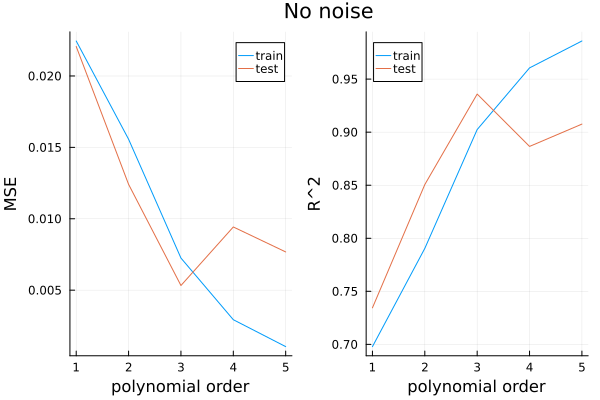
\includegraphics[scale=0.5]{linearregression_no_noise}}
    \caption{A plot of the order of polynomial features against the MSE and $R^2$ for the ols model fit. Here are using a response without stochastic noise.}
    \label{linearregression-no-noise}
\end{figure}

\begin{figure}
    \centerline{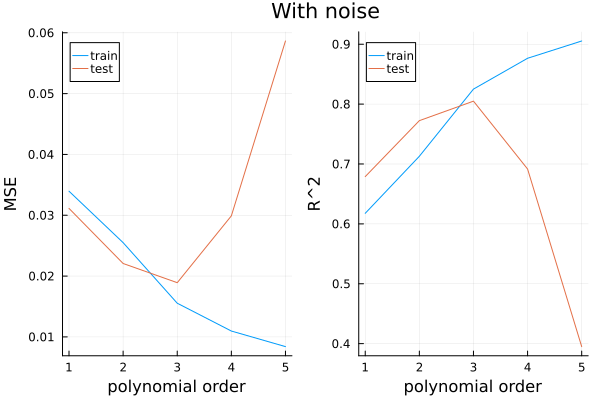
\includegraphics[scale=0.5]{linearregression_with_noise}}
    \caption{A plot of the order of polynomial features against the MSE and $R^2$ for the ols model fit. Here are using a response with stochastic noise.}
    \label{linearregression-with-noise}
\end{figure}

\begin{figure}
    \centerline{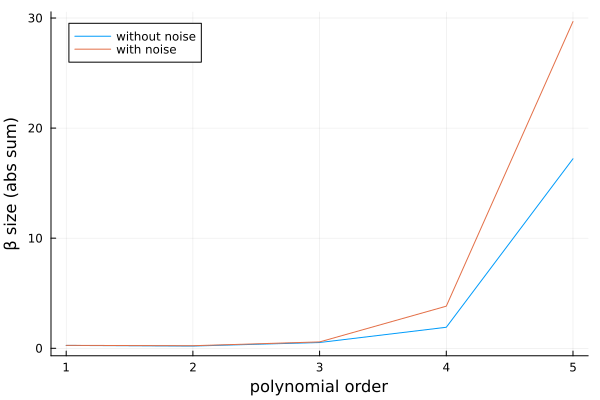
\includegraphics[scale=0.5]{linearregression_beta_size}}
    \caption{The average absolute value of our estimated $\beta$s for each polynomial order, in a ols model.}
    \label{beta-abs-sum}
\end{figure}

\subsubsection{Ridge}
If we run the \textbf{Ridge.jl} program in the project repository
\cite{githubrepoproject1} we fit the data with fifth order polynomial features
(we skip orders lower here) to ridge models with different penalization
parameter $\lambda$. From that we can extract the following
results:\\
\begin{tabular}{| c | c | c | c | c |}
          & \multicolumn{2}{|c|}{Without noise} & \multicolumn{2}{|c|}{With noise}                           \\
          & MSE                                 & $R^2$                            & MSE        & $R^2$      \\
    TRAIN & $0.001046$                          & $0.985926$                       & $0.008400$ & $0.905406$ \\
    TEST  & $0.003592$                          & $0.956765$                       & $0.017352$ & $0.821028$ \\
\end{tabular}

With the optimal $\lambda$ for test-data without noise being $1.659587\cdot
    10^{-2}$ and when we include noise it becomes $1.513561$.
To see more in detail how the MSE and $R^2$-score varies with different value of
the hyperparameter $\lambda$, see figure \ref{Lasso-no-noise} and
\ref{Lasso-with-noise}. We see that for the training-data that ridge and ols
seemingly performs almost the same.  This is because the best MSE here comes from the
lowest value of $\lambda$ (again the most complex model), which is so low that
they pretty much give the same fit. Here we see that we actually get better
performance on new data than the ols case both in the case where we have not
added noise, and when we have. In both cases these differences are quite
marginal compared to the optimal valued ols case, but still better. Keep in mind
here that we have used fifth order polynomial features, so if we compare it to
the ols case with fifth order polynomial features we get a lot better results,
especially in the case where we add noise. If we look at figure
\ref{Ridge-beta-sizes} we see that the average absolute size of our parameters
shrink as we increase $\lambda$, and hence the variance of the model also
probably will.  The fact that we manage to reduce the variance in this way is
likely the reason why our ridge model with fifth order polynomial features
vastly outperforms the ols model with the same features, at least on the
test-data when we have some added noise.
\begin{figure}
    \centerline{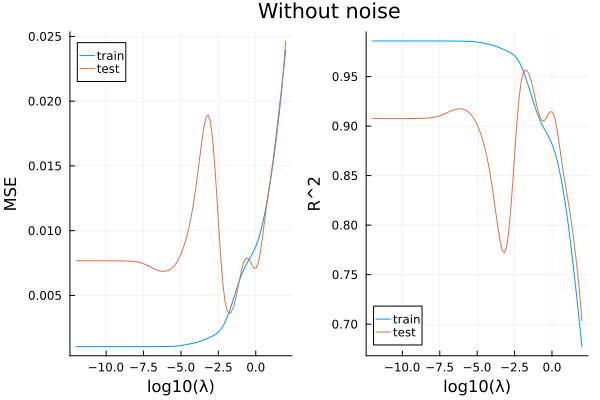
\includegraphics[scale=0.5]{ridge_without_noise}}
    \caption{A plot of the $\lambda$ in a ridge-model without noise on log10-scale plotted against the MSE and $R^2$-score. We see that performances of these metrics goes a bit up and down for the different values of $\lambda$.}
    \label{Ridge-with-noise}
\end{figure}

\begin{figure}
    \centerline{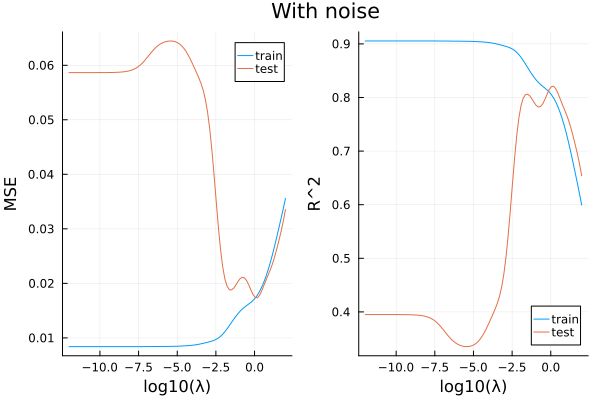
\includegraphics[scale=0.5]{ridge_with_noise}}
    \caption{A plot of the $\lambda$ in a ridge-model with $\lambda$s on log10-scale plotted against the MSE and $R^2$. We see a somewhat similar relationship as for the case with noise, but with greater scales on the y-axis for MSE.}
    \label{Ridge-no-noise}
\end{figure}

\begin{figure}
    \centerline{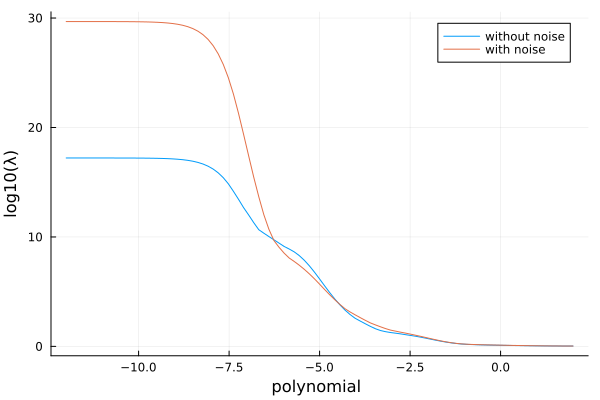
\includegraphics[scale=0.5]{ridge_beta_size}}
    \caption{The $\lambda$ plotted against the average absolute size of our parameter $\beta$. We expectedly get a shrinking relationship as we increase $\lambda$.}
    \label{Ridge-beta-sizes}
\end{figure}

\subsubsection{Lasso}
The \textbf{Lasso.jl} on the project repo \cite{githubrepoproject1} runs lasso
regression on the franke-function data and calculates the MSE and $R^2$. Running
this we can extract:

\begin{tabular}{| c | c | c | c | c |}
          & \multicolumn{2}{|c|}{Without noise} & \multicolumn{2}{|c|}{With noise}                           \\
          & MSE                                 & R\^2                             & MSE        & R\^2       \\
    TRAIN & $0.003280$                          & $0.955866$                       & $0.011319$ & $0.872539$ \\
    TEST  & $0.002737$                          & $0.967054$                       & $0.016451$ & $0.830329$ \\
\end{tabular}

With the optimal $\lambda$ for the training-data being $1.3804 \cdot 10^{-5}$, and
for the test data being $9.1201 \cdot 10^{-4}$.

In this case we get an even better performance overall than using ridge in the case of
new data, and therefore also better than the ols case, both with and without noise in
the response. One thing we notice here with the figures (\ref{Lasso-no-noise}
and \ref{Lasso-with-noise}) is that the MSE and $R^2$ scores completely flatten
out after a while. This is because when we increase the $\lambda$ enough all the
parameters will be $0$, and then all the metrics will stay the same from hereon
naturally. We also see that unlike the ridge-case the MSE and $R^2$ swings much
less in general, and almost looks to be increasing the whole way, with only a
small local/global minimums. Much like the ridge case we see from figure
\ref{Lasso-beta-sizes} that here the average parameter size also decrease when
we increase the penalization term. This indicates that as we increase the
$\lambda$ the model variance decreases, which opens up for the improvement in
MSE we have seen, again due to the bias-variance-tradeoff.

\begin{figure}
    \centerline{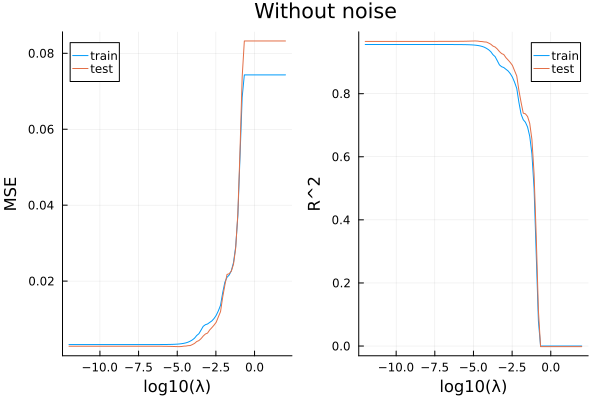
\includegraphics[scale=0.5]{lasso_without_noise}}
    \caption{A plot of the $\lambda$ in a lasso-model with $\lambda$s on log10-scale plotted against the MSE and $R^2$. Unlike the Ridge-case this completely flattens out at the end. This is due to the fact that for such high values of $\lambda$ the model-parameters which minimize the loss is simply with all the $\beta$s being $0$.}
    \label{Lasso-no-noise}
\end{figure}
\begin{figure}
    \centerline{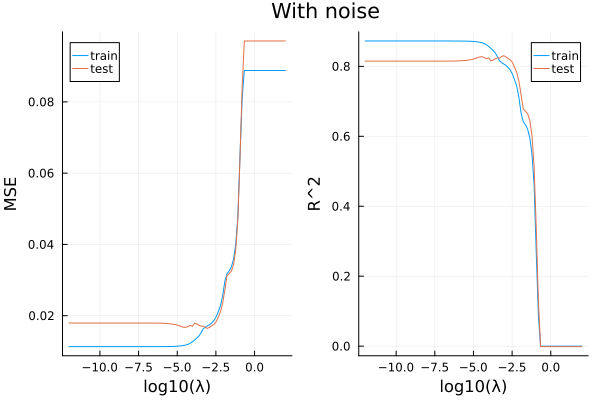
\includegraphics[scale=0.5]{lasso_with_noise}}
    \caption{A plot of the $\lambda$ in a lasso-model with $\lambda$s on log10-scale plotted against the MSE and $R^2$. We see the same flattening as in figure \ref{Lasso-no-noise}.}
    \label{Lasso-with-noise}
\end{figure}
\begin{figure}
    \centerline{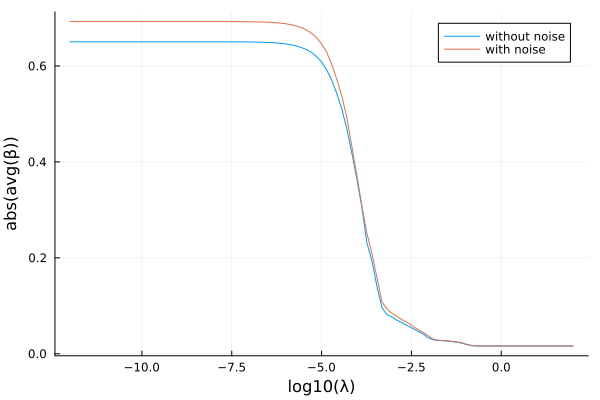
\includegraphics[scale=0.5]{lasso_beta_size}}
    \caption{$log10(\lambda)$ plotted against the average absolute size of our parameters $\beta$. We see that the relationship is expectedly shrinking.}
    \label{Lasso-beta-sizes}
\end{figure}

\subsubsection{Performance with more complex models}
Up until now we have used only polynomial features of order lower than 5. The
\textbf{Resampling.jl} and \textbf{ResamplingCV.jl} on the project repo
\cite{githubrepoproject1} explores fitting the franke-function to data with more
polynomial degrees, with the metrics calculated using bootstrap and
cross-validation respectively. Running these programs we gather some plots of
the mean squared errors plotted against the model complexity, this time in the
form of orders of polynomial features. Figure \ref{bootstrap-bias-var} shows the
mse using ols, calculated using bootstrapping, while figure \ref{crossval-ols},
\ref{crossval-ridge} and \ref{crossval-lasso} show the same graphs for ols,
ridge and lasso respectively, these calculated using cross-validation. Keep in
mind that here we have just set some fixed value for $\lambda$ for both ridge
and lasso, based on what gave good results on fifth order polynomial features in
previous calculations. Looking only at the numerical results from the
cross-validation for ols on the test-data we got:

\begin{table}[htpb!]
    \resizebox{\columnwidth}{!}{
        \begin{tabular}{| c | c | c | c | c | c | c | c | c | c | c | c | c | c |}
            Order & 2      & 3      & 4      & 5      & 6      & 7      & 8      & 9      & 10     & 11     & 12     & 13     & 14     \\
            MSE   & 0.1822 & 0.1746 & 0.1756 & 0.1796 & 0.1896 & 0.2394 & 0.4217 & 0.8437 & 1.1845 & 1.6786 & 2.0402 & 3.2349 & 4.3811
        \end{tabular}
    }
\end{table}

Similarly for ridge we got:

\begin{table}[htpb!]
    \resizebox{\columnwidth}{!}{
        \begin{tabular}{| c | c | c | c | c | c | c | c | c | c | c | c | c | c |}
            Order & 2      & 3      & 4      & 5      & 6      & 7      & 8      & 9       & 10     & 11     & 12     & 13     & 14     \\
            MSE   & 0.0172 & 0.0080 & 0.0058 & 0.0054 & 0.0055 & 0.0099 & 0.0147 & 0.02334 & 0.0364 & 0.0568 & 0.0876 & 0.1290 & 0.1830
        \end{tabular}
    }
\end{table}

And for lasso:
\begin{table}[htpb!]
    \resizebox{\columnwidth}{!}{
        \begin{tabular}{| c | c | c | c | c | c | c | c | c | c | c | c | c | c |}
            Order & 2      & 3      & 4      & 5      & 6      & 7      & 8      & 9      & 10     & 11     & 12     & 13     & 14     \\
            MSE   & 0.0169 & 0.0076 & 0.0061 & 0.0044 & 0.0036 & 0.0033 & 0.0032 & 0.0030 & 0.0029 & 0.0027 & 0.0026 & 0.0025 & 0.0025
        \end{tabular}
    }
\end{table}

\begin{figure}
    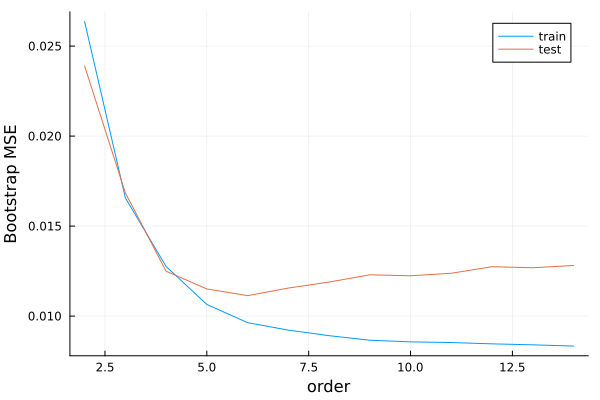
\includegraphics[scale=0.5]{bootstrapbiasvariance}
    \caption{The MSE calculated using bootstrap plotted against the increasing
        orders of polynomial features. For the training we unsurprisingly get a
        lower and lower MSE as we increase the orders of polynomials, but for the
        testing data we get at first a lower MSE by increasing the polynomials up
        until about order $6$ where it after this increases. This is to be expected
        from what we know of the bias-variance tradeoff.}
    \label{bootstrap-bias-var}
\end{figure}

\begin{figure}
    \centering
    \subfloat{{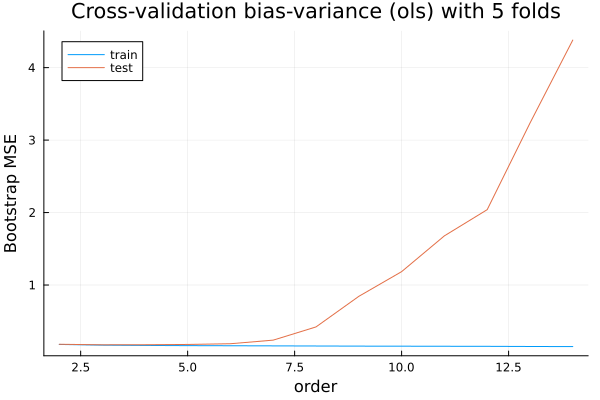
\includegraphics[width=5.5cm]{crossvalbiasvariance_ols__5_folds}}}
    \quad
    \subfloat{{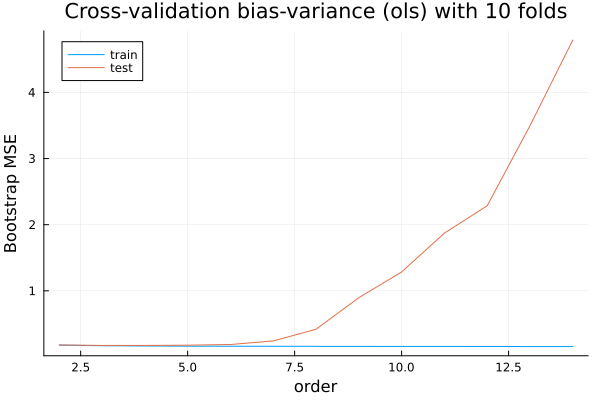
\includegraphics[width=5.5cm]{crossvalbiasvariance_ols__10_folds}}}
    \caption{Side by side cross-validated estimates of the mean squared error of
        ordinary least squares models with varying orders of features with $k=5$ and
        $k=10$ folds. We see that the mean squared error for the test data rapidly
        increases after polynomial order $\approx 6$. Since both of the results for
        $k=5$ and $k=10$ seem to be very similar we can be confident that we do not
        need to increase the amount of folds here to get a more reliable result
        - the result has already converged.}
    \label{crossval-ols}
\end{figure}
\begin{figure}
    \centering
    \subfloat{{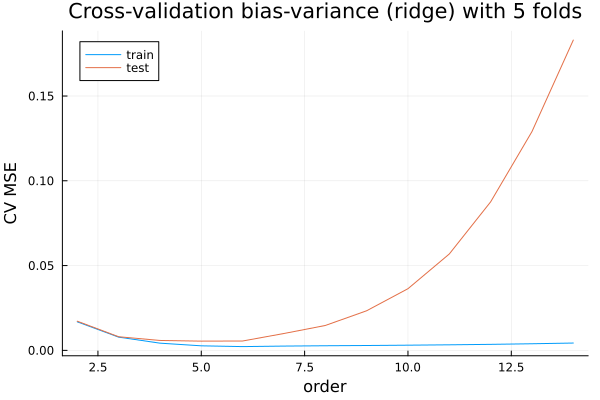
\includegraphics[width=5.5cm]{crossvalbiasvariance_ridge__5_folds}}}
    \quad
    \subfloat{{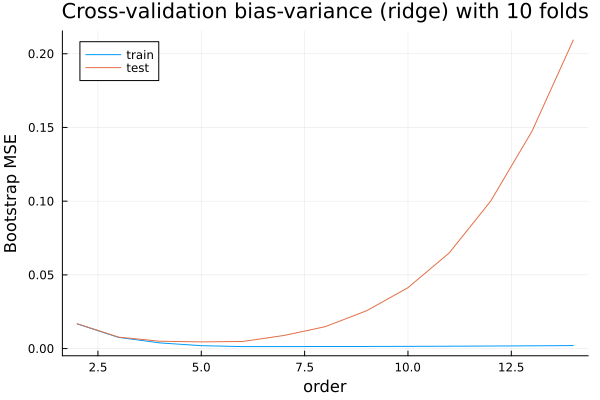
\includegraphics[width=5.5cm]{crossvalbiasvariance_ridge__10_folds}}}
    \caption{Side by side cross-validated estimates of the mse, this time for
        ridge models with varying degrees of polynomial features and $k=5$ and
        $k=10$ this time as well. We get again very similar results for the two
        sizes of folds. Here we see clearer that the test MSE decreases at first as
        we get higher order polynomial features, before it increases again as we get
        more and more complex models. We also notice that the scale here is much
        smaller than in the ols case, likely due to ridge being a less complex
        model.}
    \label{crossval-ridge}
\end{figure}

\begin{figure}
    \centering
    \subfloat{{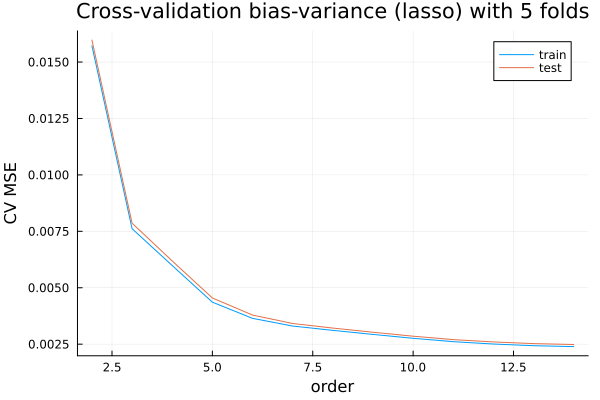
\includegraphics[width=5.5cm]{crossvalbiasvariance_lasso__5_folds}}}
    \quad
    \subfloat{{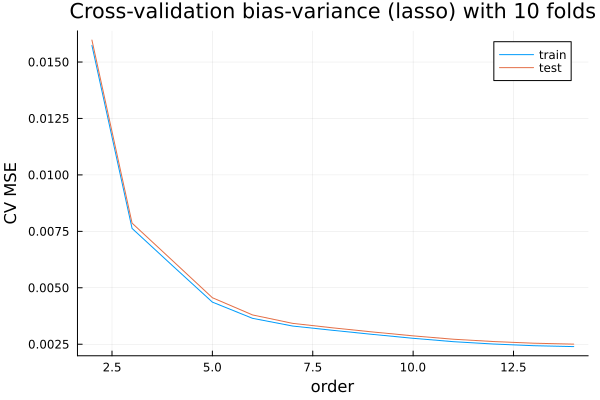
\includegraphics[width=5.5cm]{crossvalbiasvariance_lasso__10_folds}}}
    \caption{Side by side cross-validated estimates of the mse, finally this time for lasso models with varying degrees of polynomial features and $k=5$ and
        $k=10$ folds this time as well, with the same result for the two
        different fold sizes. Interesting here is that we actually get better
        and better performance as we increase the polynomial order it could look
        like. Keep in mind though that we only have tested up to order $14$. If
        we were to increase this even more, we likely would get problems so long
        as the $\lambda$ parameter stays the same.}
    \label{crossval-lasso}
\end{figure}

Here we can see the bias-variance tradeoff in full effect. When we include
higher order polynomial features, we also get a higher model-complexity. This
means our models will have lower bias, but also much higher variance. The
expected prediction error being the sum of these two typically means that our
model-performances follows a sort of U-shape plotted against model-complexity
(this we have already seen for the ols and ridge MSE plots in particular),
where the optimal value has a somewhat low bias and a somewhat low variance, but
also typically not at the minimum of either. This is what we see in general
throughout our results here (see figure \ref{bootstrap-bias-var} and
\ref{crossval-ridge} in particular). From our results it seems that for ridge
and ols, that there is not much point going beyond fifth order polynomial
features. Here the exception seems to be the Lasso, which seems to only get a
lower and lower MSE as we increase the polynomial order.  This is probably
partially because lasso is able to perform its own kind of model-selection,
where the parameter corresponding to some of the features will be $0$. However
if we add more and more polynomial features and still keep the $\lambda$ fixed,
we would eventually get an increase in the MSE as the lasso would not be able to
reduce the variance enough to keep up with the more and more complex features.

\subsection{Landscape data}
Running the \textbf{Landscape.jl} on the project repo \cite{githubrepoproject1}
we perform cross-validation on the various models to estimate MSE, and choose
the optimal hyperparameters. We here kept to polynomial features of order $5$
which seemed to get us quite good performance across the models for the
franke-function (perhaps with the exception of ols, but keep in mind that we
have much more data here). When using the ols and calculating the MSE using
cross-validation we get a MSE value of $\approx 1.6075\cdot 10^{-5}$, and when
evaluating on the separate test-data we get $\approx 1.5878 \cdot 10^{-5}$. For
ridge regression we use the cross-validation to determine the optimal $\lambda$
we get this to be $\approx 4.6416 \cdot 10^{-8}$, with a corresponding MSE to
of $\approx 1.6 \cdot 10^{-5}$, much like the ols case. Evaluated on the
test-set for this model we get a MSE of $\approx 1.5878 \cdot 10^{-5}$. For
lasso we get the optimal $\lambda$ to be $10^{-10}$, which is the smallest
possible value, with a corresponding MSE to be $\approx 2.4 \cdot 10^{-5}$. On
the test-data this MSE was $\approx 2.37 \cdot 10^{-5}$.
\\
What is noticeable here is that we get the best $\lambda$ values for prediction
for both the ridge and lasso to be very low, meaning we do not get a lot of
reduction in the parameters, and therefore also not much reduction in model variance. This
is likely because we have a lot more data-points in this case so the
model-variances become rather small in all cases, so there is not much to gain
from reducing this further, and therefore the models with lower bias will give
the best predictions (which is the ols).

\section{Analysis}
As we can see from the results, in the case when we have data without noise
(as in the franke-function with no noise), we have quite comparably good results
when fitting the different models to the data, with lasso performing just about
better than ridge, while ols performing the worst, but still quite good. When we
add noise to the data all the models perform worse, but lasso and ridge manage
to still come up with quite good performance (lasso still performed the best),
while higher order polynomial featured ols (the most complex models) performed
much much worse than before, but lower order ols models performed comparable to
ridge/lasso still.  What ridge and lasso models with quite big values of
$\lambda$ and lower order polynomial ols have in common is that they are all
comparatively not that complex models. The reason these models performed so good
is likely because, even though the model bias is somewhat bigger, the variance
will be much smaller, and from the bias-variance-tradeoff we know that it is the
sum of these which needs to be low for the model to make good predictions. We
have seen this also when trying out different polynomial orders and seeing the
MSE values these give. In general at least for ridge and ols we see that both
calculating the MSE using bootstrap and cross-validation that we get slight
decreases in MSE when increasing the polynomial orders, before the MSE
eventually increase again with the polynomial order as the models get more
complex. Looking at the overall performances for the different models on the
different polynomial orders we see that they all work the best on quite
different orders. For the ridge one would get the best performance around $5$-th
order polynomial features, while for ols this is closer to $3$-rd order, while
for lasso one can go a lot higher than both of the ols and ridge.  For the
landscape data we saw that we got a similar performance for the ols and ridge,
while lasso all of a sudden performed the worst. This difference is likely
related to a different signal-to-noise-ratio than before, but perhaps even more
important, due to the fact that we then had many more observations. With more
observations we do not overfit like we did before, and the variance of the model
becomes lower than when we had less data.  This makes linear regression a more
viable choice seeing as this often has considerably lower bias.\\ At last, one
thing to take note of is that throughout some of the code (in particular the
parts that have to do with ridge/lasso using the franke-function), we have
fitted many models with different hyperparameters and then chosen the model
which gave the best result for our MSE metric. This MSE metric however would be
too optimistic for the MSE on the true data \cite[s.~7.2]{hastie2009elements}.
Here we could further improve the estimates by generating a separate test-set,
which we evaluate our selected best model on.  Keep in mind though that we did
do this for the landscape data, so our metrics here should be rather fine.
Another place we could improve is to test performances for more penalization
terms for ridge and lasso. We used a limited set here in order to speed up the
calculations, and one could perhaps test a few more in order to see if
model-performances becomes better. Likewise one could also test higher/lower
order polynomial features for the models of the landscape-data, and see if we
can get better performance on a polynomial order other than $5$.

\section{Conclusion}
We have in this project seen how ols, ridge and lasso performs on data generated
from the franke-function and landscape-data. We see that for data without noise
and quite low amount of observations, that all these three different models
performed somewhat similarly, but when we added noise that the less
complex models, i.e. ridge and lasso with a sizeable $\lambda$ parameter,
and ols with lower order polynomial features performed better. This clearly is
related to the bias-variance-tradeoff, which we have derived earlier. However in
the case of the landscape-data, where we had a lot more observations and
polynomial features of order five, the ols performed much better, and the
ridge/lasso with $\lambda$ parameters of any meaning performed worse. Over the
two datasets we have manifested the importance of choosing models of right
model-complexity in order to get the best predictions. We also saw that using
models with lower variance became important when we had few observations and a
sizeable amount of noise, but less important when we have a good amount of
observations and no/tiny stochastic noise in the data.

\section{Appendix}

\subsection{Project code (github)}
All the Julia programs described in the report and with the full source code can be
found at:
\url{https://github.com/magnouvean/ml-physics-projects/tree/main/project1/julia}

\subsection{Expectance and variance with matrices}
Let $A$ be a non-stochastic $p \times n$ matrix and $\mathbf{X}$ be a stochastic
$n \times 1$ vector. We have:
$$E(A \mathbf{X}) = (E((A \mathbf{X})_1), \dots, E((A \mathbf{X})_p))^T$$
We then have:
$$E(A \mathbf{X})_i = E((A \mathbf{X})_i) = E(\sum_{k=1}^n A_{i k} \mathbf{X}_k) = \sum_{k=1}^n A_{i k} E(\mathbf{X}_k) = A_{i *} E(\mathbf{X})$$
Hence we see that $E(A \mathbf{X}) = A E(\mathbf{X})$.
Note also that from this it follows that $E(A \mathbf{X})^T = (A
    E(\mathbf{X}))^T = E(\mathbf{X})^T A^T$ (we will use this for calculating the
variance expression).

We now want to look at the case of the variance. We first calculate an
intermediate expression. Let $A$ as before be a non-stochastic $p \times n$
matrix and $\mathbf{B}$ a stochastic $n \times n$ matrix. We want to find:
$$E(A \mathbf{B} A^T)$$
We have:
\begin{align*}
    E(A \mathbf{B} A^T)_{i j} & = E((A \mathbf{B} A^T)_{i j})                                         \\
                              & = E(\sum_{k = 1}^n A_{i k} (\mathbf{B} A^T)_{k j})                    \\
                              & = \sum_{k = 1}^n A_{i k} E((\mathbf{B} A^T)_{k j})                    \\
                              & = \sum_{k = 1}^n A_{i k} E(\sum_{l=1}^{n} \mathbf{B}_{k l} A^T_{l j}) \\
                              & = \sum_{k = 1}^n A_{i k} \sum_{l=1}^{n} A^T_{l j} E(\mathbf{B}_{k l}) \\
                              & = (A E(\mathbf{B}) A^T)_{i j}
\end{align*}
Hence we see that $E(A \mathbf{B} A^T) = A E(\mathbf{B}) A^T$.  We are now ready
to find the variance:
\begin{align*}
    Var(A \mathbf{X}) & = E((A \mathbf{X} - E(A \mathbf{X})) (A \mathbf{X} - E(A \mathbf{X}))^T)                                                                       \\
                      & = E((A \mathbf{X})(A \mathbf{X})^T  - A \mathbf{X} E(A \mathbf{X})^T - E(A \mathbf{X}) (A \mathbf{X})^T + E(A \mathbf{X}) E(A \mathbf{X})^T)   \\
                      & = E(A \mathbf{X}\mathbf{X}^T A^T  - A \mathbf{X} E(\mathbf{X})^T A^T - A E(\mathbf{X}) \mathbf{X}^T A^T + A E(\mathbf{X}) E(\mathbf{X})^T A^T) \\
                      & = E(A (\mathbf{X}\mathbf{X}^T  - \mathbf{X} E(\mathbf{X})^T - E(\mathbf{X}) \mathbf{X}^T + E(\mathbf{X}) E(\mathbf{X})^T ) A^T)                \\
                      & = A E((\mathbf{X} - E(\mathbf{X})) (\mathbf{X} - E(\mathbf{X}))^T) A^T                                                                         \\
                      & = A Var(\mathbf{X}) A^T                                                                                                                        \\
\end{align*}
Where we have used the previous result for the second last equality.

\bibliography{./sources.bib}

\end{document}